\section{Motivations}
A volumetric display is a type of graphical display device that can provide a visual representation of objects natively in 3D. They can be viewed from any angle without the need for special visual apparatus by multiple people simultaneously \cite{1492264}. These displays differ from more traditional virtual reality devices in that they are not immersive, but rather they are a window into a virtual world (See Fig~\ref{fig:passive-optical} and Fig~\ref{fig:acoustic}). There is no real consensus on what exactly constitutes a volumetric display, let alone the best way to build one. As we cover in the background section there are currently many approaches being attempted by research groups both academic and industrial to create these displays. 
 
\begin{invisBox}
\pictureBox[label={fig:passive-optical}]{Columbia University's passive optical scattering volumetric display \cite{10.1145/1179849.1179982}}{
  \adjustbox{height=5.25cm, keepaspectratio}{
    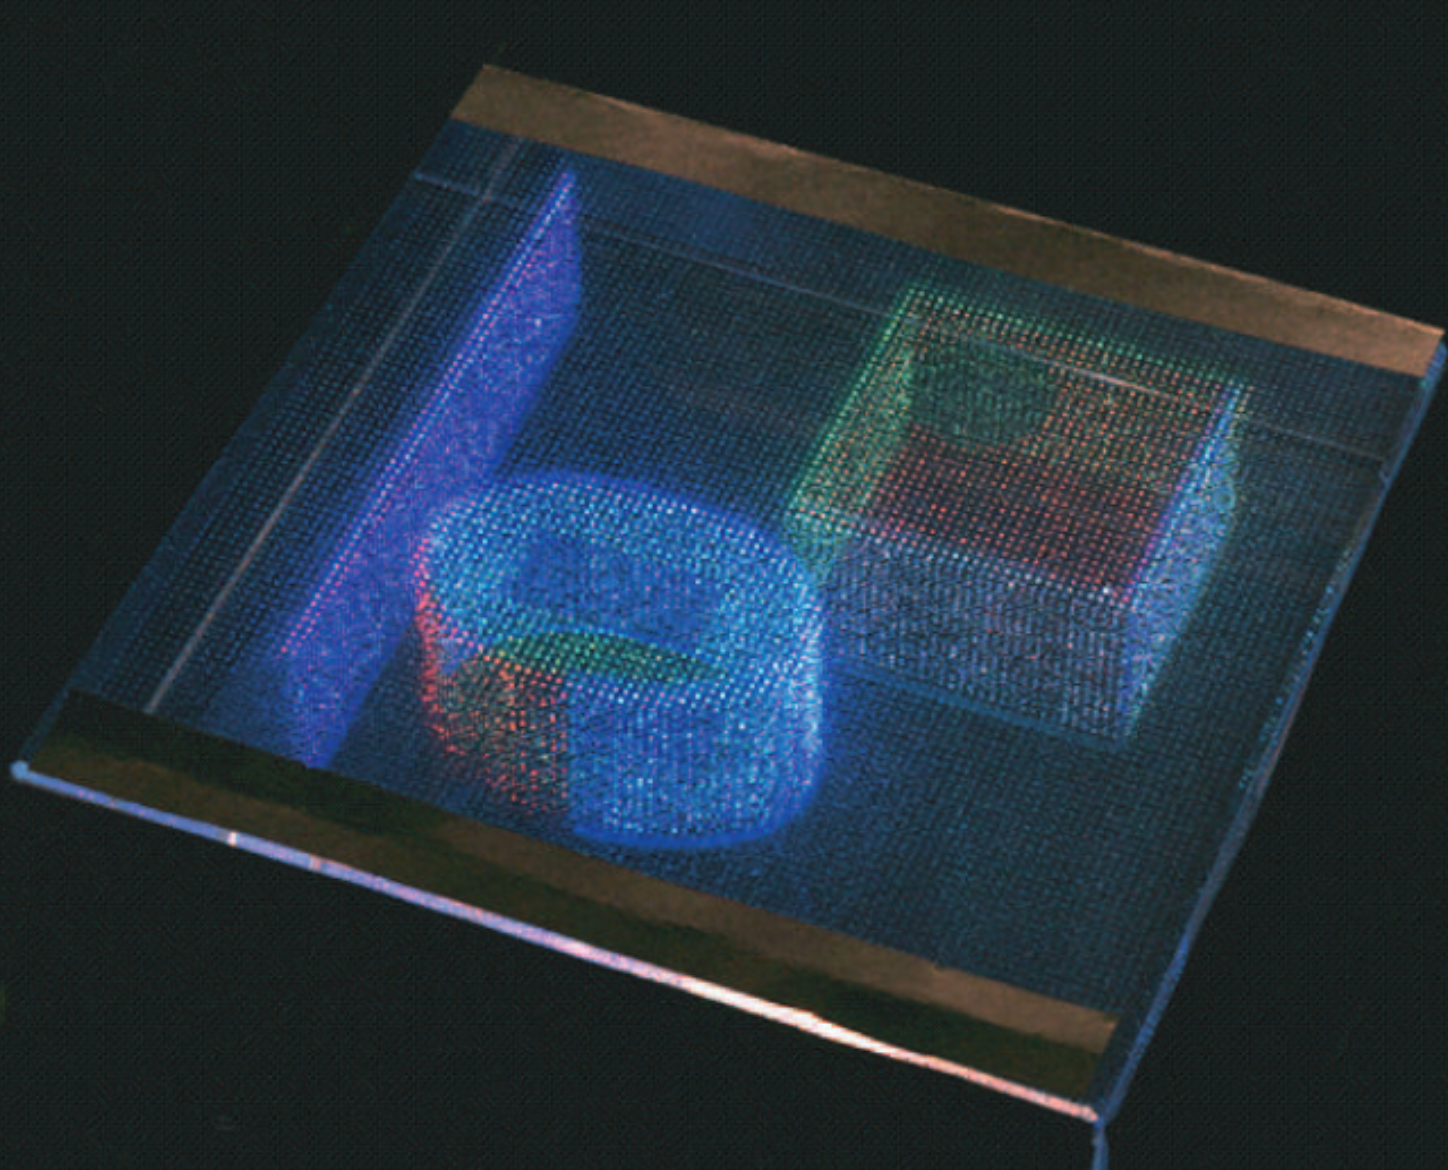
\includegraphics{./introduction/figures/passive optical scatterers.png}
  }
}
\hfill
\pictureBox[label={fig:acoustic}]{Bristol University's acoustic trapping volumetric display \cite{10.1063/1.5113467}}{
\adjustbox{height=5.75cm, keepaspectratio}{
  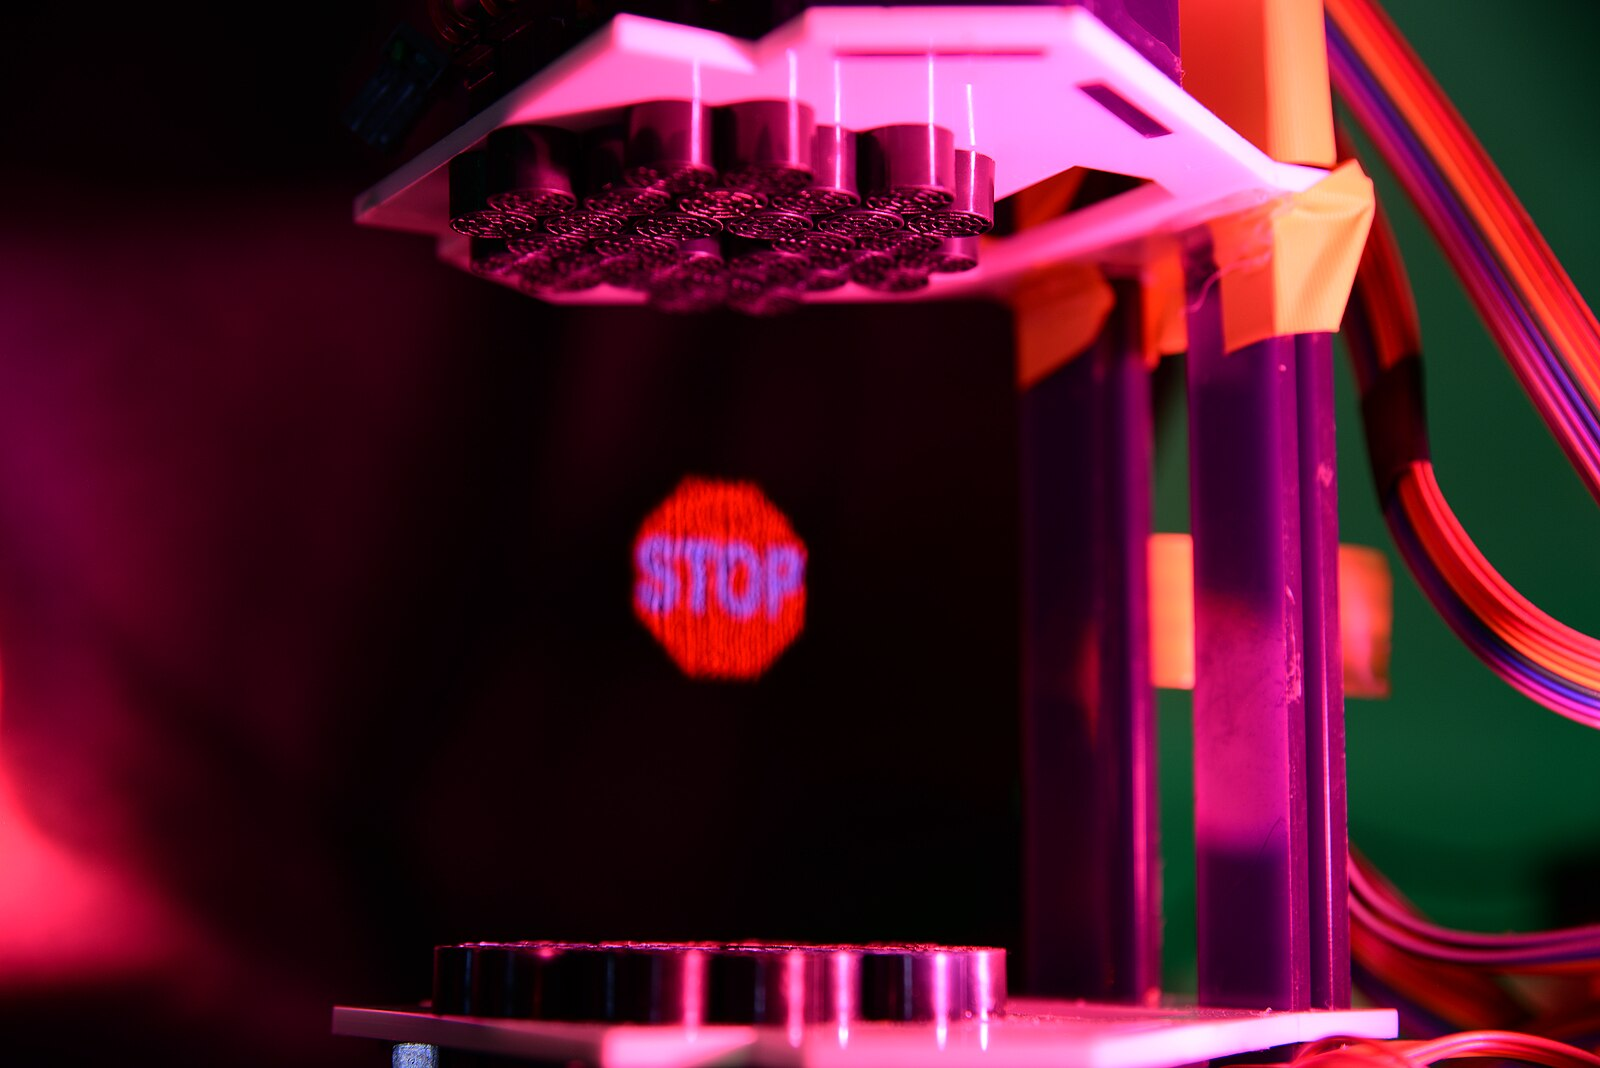
\includegraphics{./introduction/figures/acoustophoretic display.jpg}
  }
}
\end{invisBox}

At the time of writing it is difficult to conduct human-computer interaction (HCI) research into the field of volumetric displays because these devices are not widely available, expensive and difficult to manufacture, and have extreme bandwidth requirements which makes it difficult to conduct user studies and experiments. People have created virtual simulations of volumetric displays before to try and solve this problem, but these solutions are often complicated and expensive to replicate.

\textcolor{red}{explain how expensive they are}

\textcolor{red}{explain uses of volumetric displays vs VR}

\section{Contributions}

Our project makes two novel contributions to the field of volumetric displays. Firstly we built a system for accurately simulating Volumetric Displays. Secondly we ran a successful user study utilizing our device showing the research viability of our system. 

\textcolor{red}{Add Images of display}

\subsubsection{Volumetric Display Simulator}
We created our Volumetric Display Simulator (See \ref{sect:overview}) with the intention of creating strong foundation for running user studies involving Volumetric Displays. We designed our system in a such a way that it is: 

\begin{enumerate}
    \item \textbf{Cost-Effective:} The system was designed to operate on a standard desktop computer with standard monitors using common hardware and utilizes Microsoft's widely used Azure Kinect Camera. We believe our system's affordability and accessibility will encourage more researchers to explore volumetric display technology.

    \item \textbf{Reproducible:} The system was developed using Nix (See \ref{sect:nix}), a package manager that facilitates the easy reproduction and compilation of the software environments. This means the system can be run on any computer with Nix installed using a single command. This not only simplifies execution but also enhances the ease of sharing and reproducing results.

    \item \textbf{Simple and Lightweight:} The system was intentionally designed to be as simple as possible by leveraging well-established libraries (See \ref{sect:renderer} and \ref{sect:tracker}). The simulator comprises only approximately 2,000 lines of C++ code, making it straightforward to understand and modify. The use of Nix to manage the environment ensures that the system can be deployed with a single command, further enhancing its accessibility and usability (See \ref{sect:buildsystem}).
\end{enumerate}

\subsubsection{User Study}

We ran a user study to successfully validate the effectiveness of our volumetric display system. We investigated the difference in performance of a task using your hands between 2D and 3D viewing perspectives on our display, and the effect of teleoperation, offsetting the display from the zone where the participant interacts with the task (See \ref{sect:userstudy}). \\

The findings indicated that using a 3D tracking mode significantly improves task completion speed and accuracy compared to a traditional 2D static display. Additionally, direct hand interaction with the volumetric display yielded superior results compared to teleoperation, particularly in 3D scenarios. These outcomes underscore the importance of depth perception and natural interaction in maximizing the usability and performance of volumetric displays. \\

This research makes several key contributions to the field of human-computer interaction and volumetric display technology:

\begin{itemize}
    \item \textbf{Empirical Validation:} The study provides empirical evidence that 3D volumetric displays, when used with direct hand interaction and without offset, significantly enhance task performance. This contributes to the body of knowledge regarding the practical benefits of volumetric displays over traditional 2D interfaces.

    \item \textbf{Insight into Motion Parallax:} The findings reaffirm the critical role of motion parallax in 3D display interactions. By showing that the benefits of 3D tracking are diminished with positional offsets, the study offers valuable insights into the design and application of volumetric displays, suggesting that maintaining a consistent perspective is crucial for effective use.

    \item \textbf{User Preference Analysis:} The strong user preference for 3D tracking conditions underscores the importance of user-centered design in developing interactive systems. This preference suggests that users value intuitive and natural interaction modes, which should be a priority in future interface designs.

    \item \textbf{Recommendations for Future Research:} The study identifies several areas for further investigation, including the effects of varying offset distances and the potential impact of offsetting the interaction zone rather than the display itself. These recommendations can guide future research efforts to refine and improve the usability of volumetric displays.
\end{itemize}
